\documentclass{beamer}
\mode<presentation>{
  \usetheme[compress]{Berlin}
}

%% packages
\usepackage{zhspacing}
\zhspacing
\usepackage{graphics}
\usepackage{subfigure}
\usepackage{multirow}
\usepackage{listings}
\lstset{basicstyle=\ttfamily\small}
%% meta info
\title{Rat: 一种函数式并行程序语言}
\author[苏醒~pysuxing@gmail.com]{
\begin{tabular}{ll}
答辩人: & 苏醒 \\
指导教师: & 窦文华~教授
\end{tabular}
}
\institute{计算机所641教研室}
\date{2013-10-22}

%% slides
%% cover and content
\begin{document}
\setlength{\parindent}{0pt}
\begin{frame}
  \titlepage
\end{frame}

\begin{frame}
  \tableofcontents
\end{frame}

%% chap 1
\section{研究内容}
\frame{\tableofcontents[currentsection]}
\begin{frame}
  \frametitle{研究内容}
  本课题研究点主要包括:
  \begin{itemize}
    \item 并行程序语言的语法设计
      \begin{itemize}
        \item 定位:Domain Specific Language
        \item 目标:在保证效率的前提下提高易用性
        \item 内容:类型系统,表达式种类,高阶特性
      \end{itemize}
      \pause
    \item 语言的实现技术
      \begin{itemize}
        \item Runtime System:为内存管理、线程管理、任务划分等并行细节提供支持
        \item 异构硬件的利用:CPU与GPU的协同工作
        \item 优化措施:存储器优化以及GPU片上共享存储器的优化
      \end{itemize}
  \end{itemize}
\end{frame}

%% chap 2
\section{语言设计}
\frame{\tableofcontents[currentsection]}
\subsection{引子:并行问题实例}
\frame{\tableofcontents[currentsection, currentsubsection]}
\begin{frame}[t]
  \frametitle{并行程序设计实例:向量内积}
  考虑一个经典数据并行问题:
  \begin{block}{向量内积}
    $d=u \cdot v = \sum_{k=1}^nu_kv_k$
  \end{block}

  \only<2>{
    %% \begin{block}{C语言顺序实现}
    C语言顺序实现
    \lstinputlisting[language=C]{listings/dot-c.c}
    %% \end{block}
  }
  \only<3>{
    %% \begin{block}{Rat实现}
    Rat实现
    \lstinputlisting[language=Haskell]{listings/dot-rat.hs}
    %% \end{block}
  }
\end{frame}

\subsection{类型系统}
\frame{\tableofcontents[currentsection, currentsubsection]}

\begin{frame}
  \frametitle{Rat的数据类型}
  Rat 采用静态数据类型系统,执行编译期类型检查(FIXME:这里的举例结合矩阵乘法的例子)
  \begin{itemize}
    \item 标量类型
      \begin{itemize}
        \item 定长整数\\ \texttt{(U)Int8, (U)Int16, ... (U)Int64, (U)Int}
        \item 浮点数\\ \texttt{Float, Double}
      \end{itemize}
    \item 向量类型\\
      \texttt{[e]}包含元素类型为\texttt{e}(标量类型)的向量类型
    \item 结构类型\\
      \text{(Int32, Double ...)}
    \item 函数类型\\
      从\texttt{Int32}到\texttt{Int32}的函数类型~\texttt{Int32 -> Int32} 
  \end{itemize}
\end{frame}

\begin{frame}
  \frametitle{多态---type class}
  Rat 支持 type class,即某一类具有共同性质的数据类型。支持多态可以避免为不同类型的数据
  分别定义相同的操作。
  \begin{itemize}
    \item 数值类型 Numeric
      \lstinputlisting[language=Haskell]{listings/frag-3.hs}
    \item 幺半群类型
      \lstinputlisting[language=Haskell]{listings/frag-4.hs}
  \end{itemize}
  \pause
  %% \begin{block}{recall: C++ template}
  recall: C++ template
  \lstinputlisting[language=C++]{listings/cpp-template.cpp}
  %% \end{block}
\end{frame}

\begin{frame}
  \frametitle{type class实例}
  以0为幺元,加法运算为结合律二元运算的 Float 上的幺半群
  \lstinputlisting[language=Haskell]{listings/frag-1.hs}
  \pause
  type class的另一作用:为可并行化操作提供约束。
  \lstinputlisting[language=Haskell]{listings/frag-2.hs}
\end{frame}

\subsection{函数式语言特性}
\frame{\tableofcontents[currentsection, currentsubsection]}
\begin{frame}
  \frametitle{函数式语言特性}
  \begin{itemize}
    \item “一等公民”(first-class citizen)
    \item 纯函数特性(pure functional)
    \item 柯里化(curried)
    \item 恒值对象(immutable object)
  \end{itemize}
\end{frame}

\begin{frame}
  \frametitle{函数式语言特性}
  \framesubtitle{“一等公民”}
  函数可以是
  \begin{itemize}
    \item<1-> 其他函数的参数
      \lstinputlisting[language=Haskell]{listings/frag-5.hs}
    \item<2-> 函数的返回值\\
      \lstinputlisting[language=Haskell]{listings/frag-6.hs}
    \item<3-> 匿名函数(lambda表达式)\\
      \lstinputlisting[language=Haskell]{listings/frag-7.hs}
  \end{itemize}
\end{frame}

\begin{frame}
  \frametitle{函数式语言特性}
  \framesubtitle{纯函数特性(pure functional)}
  也称“无副作用”(side-effect free),即只要给定同样的输入,就得到同样的输出。
  side-effect free 可以大大简化程序语义的分析。
  \begin{itemize}
    \item 纯函数举例:\\\texttt{sqrt, pow, exp ...}
    \item 副作用函数:\\\texttt{printf, readline ...}
  \end{itemize}
\end{frame}

\begin{frame}
  \frametitle{函数式语言特性}
  \framesubtitle{柯里化(curried)}
  \begin{itemize}
    \item<1-> 函数的形式参数支持部分实例化。
      \lstinputlisting[language=Haskell]{listings/frag-8.hs}
    \item<2-> 另一种视角:将n元函数看作一个1元函数,该1元函数的返回类型是一个(n-1)元函数
      \lstinputlisting[language=Haskell]{listings/frag-9.hs}
  \end{itemize}
\end{frame}

\begin{frame}
  \frametitle{函数式语言特性}
  \framesubtitle{恒值对象(immutable object)}
  无赋值操作,一个对象只在被定义的时候赋值,并在之后的生命周期中不再变更
  \lstinputlisting[language=Haskell]{listings/frag-10.hs}
\end{frame}

\begin{frame}
  \frametitle{函数式语言的优势}
  为什么采用函数式语言设计?
  \begin{itemize}
    \item 语义精确,容易分析\\
      数值计算领域关注计算,满足“side-effect free”的要求
    \item 描述问题本身的求解,隐藏计算机实现细节
  \end{itemize}
  \pause
  其他编程范式
  \begin{itemize}
    \item 过程式(命令式)语言\\
      抽象级别低,细节隐藏差
    \item 对象式语言\\
      应用于数值计算领域无优势
  \end{itemize}
\end{frame}

\subsection{编程界面}
\frame{\tableofcontents[currentsection, currentsubsection]}
\begin{frame}
  \frametitle{编程界面}
  Rat语言包括两类数据操作:
  \begin{itemize}
    \item<1-> 标量操作~Scalar Operation(SOP)
      \begin{itemize}
        \item 标量原语Scalar Primitive(SP):基本的算数逻辑运算\\
          \texttt{+, -, *, /, mod, exp, sqrt, ...}
        \item 用户自定义标量函数
      \end{itemize}
    \item<2-> 向量操作Vector Operation(VOP)
      \begin{itemize}
        \item 向量原语Vector Primitive(VP)\\
          \texttt{map, scan, permute, slice, compact, sparse, sort, zip, random}
        \item 用户自定义向量函数
      \end{itemize}
  \end{itemize}
\end{frame}

\begin{frame}[t]
  \frametitle{向量原语}
  向量原语是并行数据操作的核心
  \only<1>{
    \begin{figure}
      \caption{map}
      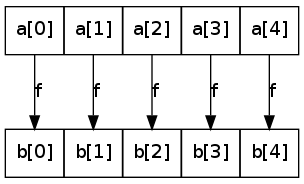
\includegraphics[scale=0.4]{images/map.png}
    \end{figure}
  }
  \only<2>{
    \begin{figure}
      \caption{compact}
      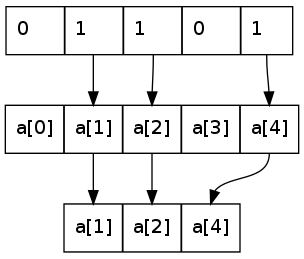
\includegraphics[scale=0.4]{images/compact.png}
    \end{figure}
  }
  \only<3>{
    \begin{figure}
      \caption{sparse}
      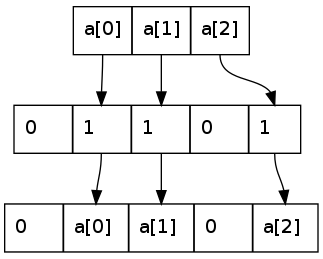
\includegraphics[scale=0.4]{images/sparse.png}
    \end{figure}
  }
  \only<4>{
    \begin{figure}
      \caption{permute}
      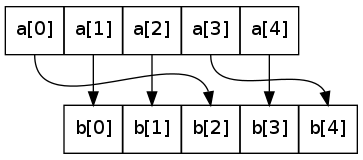
\includegraphics[scale=0.4]{images/permute.png}
    \end{figure}
  }
  \only<5>{
    \begin{figure}
      \caption{zip}
      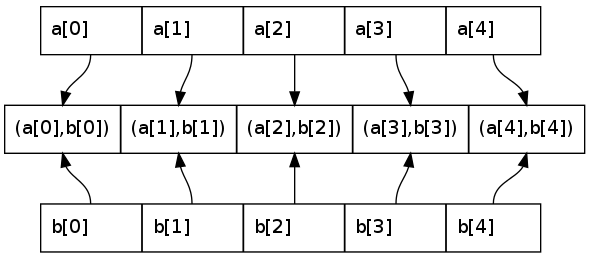
\includegraphics[scale=0.4]{images/zip.png}
    \end{figure}
  }
\end{frame}

\begin{frame}
  \frametitle{一个完整实例}
  n-body问题
  \lstinputlisting[language=Haskell, basicstyle=\ttfamily\scriptsize]{listings/nbody.hs}
\end{frame}

\begin{frame}
  \frametitle{小结:Rat语言的语法特点}
  \begin{itemize}
    \item 高层的编程界面,数学化的程序表达,适用于数据并行编程问题
    \item 细节隐藏,消除内存管理、线程管理、消息传递等编程复杂性
    \item 强静态类型系统,极大降低运行期错误发生的可能性
  \end{itemize}
\end{frame}

%% chap 3
\section{实现技术}
\frame{\tableofcontents[currentsection]}
\subsection{前端处理流程}
\frame{\tableofcontents[currentsection, currentsubsection]}
\begin{frame}
  \frametitle{源程序分析}
  \framesubtitle{level-1~语法树}
  level-1 语法树即为源程序树,包括以下结点类型:
  \begin{table}
    \caption{level-1 语法树的结点类型}
    \begin{tabular}{|l|l|l|}
      \hline
      type-def & variable-decl & variable-def\\
      \hline
      literal & variable-ref & function-app\\
      \hline
      lambda-exp & conditional & vector-comprehension\\
      \hline
      vector-element-ref & vector-slice-ref & local-binding\\
      \hline
    \end{tabular}
  \end{table}
\end{frame}

\begin{frame}
  \frametitle{源程序分析}
  \framesubtitle{level-2~语法树}
  由 level-1 语法树变换得到的 level-2 语法树结构更为简化。
  \begin{table}
    \caption{level-2 语法树的结点类型}
    \begin{tabular}{|l|l|l|}
      \hline
      literal & variable-ref & function-app\\
      \hline
      lambda-exp & conditional &\\
      \hline
    \end{tabular}
  \end{table}
\end{frame}

\begin{frame}
  \frametitle{Core语言}
  Rat核心语言Core,将 level-2 语法树中的柯里化(curried)函数变换为
  反柯里化(uncurried)形式。程序的优化与翻译在Core语言上执行。
\end{frame}

\begin{frame}
  \frametitle{Core语言}
  \begin{block}{实例:求解向量内积}
    \lstinputlisting[language=Haskell]{listings/frag-11.hs}
  \end{block}
  \begin{figure}
    \caption{level-2语法树到Core语言语法树的变换}
    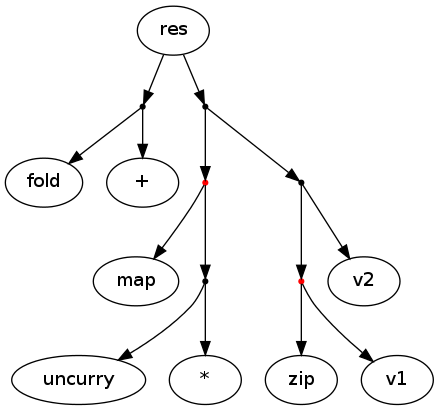
\includegraphics[scale=0.2]{images/level-2-tree.png}
    \pause
    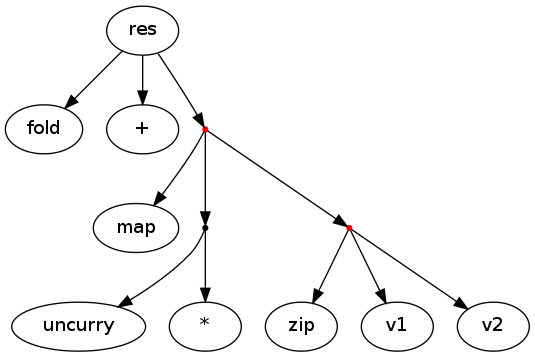
\includegraphics[scale=0.2]{images/core-tree.png}
  \end{figure}
\end{frame}

\begin{frame}
  \frametitle{Core语言的翻译}
  Core语言运行于Rat虚拟机之上。Rat虚拟机抽象层次较高,它的基本
  指令由Rat的内建标量函数与向量原语VP组成。
  \begin{itemize}
    \item 标量原语SP\\
      \texttt{+, -, *, /, mod, exp, sqrt, ...}
    \item 向量原语VP\\
      \texttt{map, scan, permute, slice, compact, sparse, sort, zip, random}
  \end{itemize}
\end{frame}

\begin{frame}
  \frametitle{Core语言的翻译}
  \begin{block}{实例:求单精度浮点复数的模}
    $C=x+yi$\hspace{3cm}$\Vert C \Vert = \sqrt{x^2+y^2}$
  \end{block}
  \pause
  \lstinputlisting[language=Haskell]{listings/frag-15.hs}
  \pause
  \begin{figure}
    \caption{复数求模函数的Core树}
    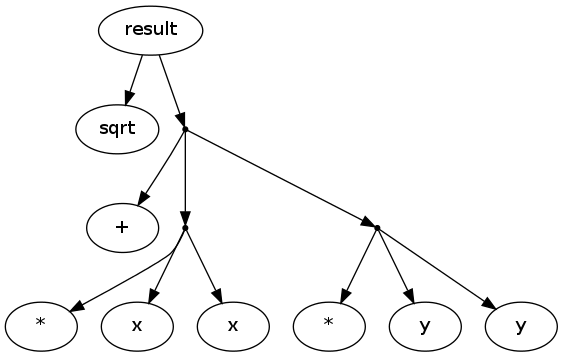
\includegraphics[scale=0.2]{images/complex-length.png}
  \end{figure}
\end{frame}

\begin{frame}[t]
  \frametitle{Core语言虚拟机}
  以原语操作为基本指令的虚拟机。

  \only<1>{
    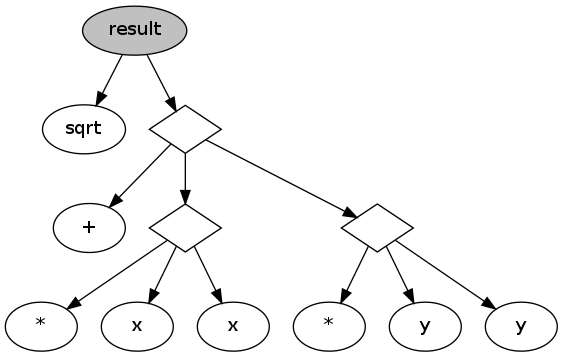
\includegraphics[scale=0.25]{images/vm-1.png}
    \hspace{.3in}
    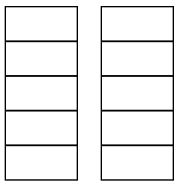
\includegraphics[scale=0.5]{images/stack-1.png}
  }
  \only<2>{
    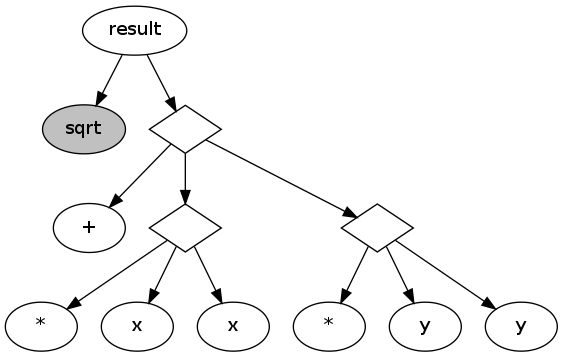
\includegraphics[scale=0.25]{images/vm-2.png}
    \hspace{.3in}
    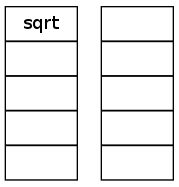
\includegraphics[scale=0.5]{images/stack-2.png}
  }
  \only<3>{
    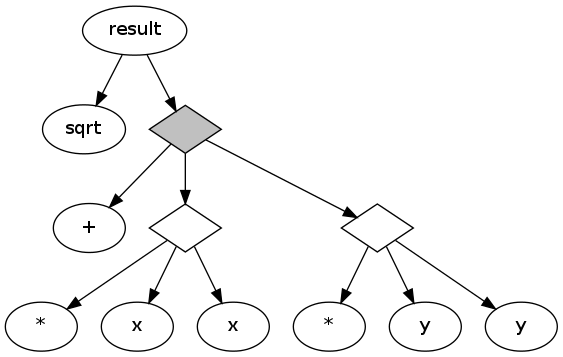
\includegraphics[scale=0.25]{images/vm-3.png}
    \hspace{.3in}
    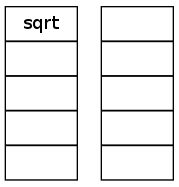
\includegraphics[scale=0.5]{images/stack-2.png}
  }
  \only<4>{
    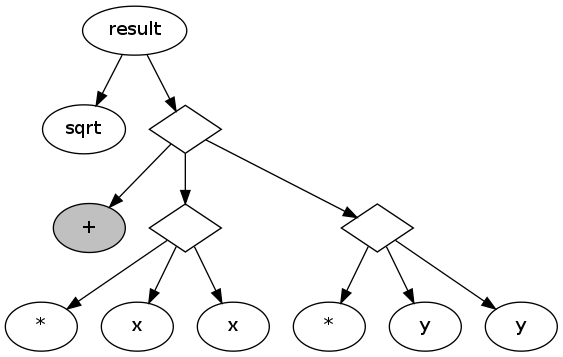
\includegraphics[scale=0.25]{images/vm-4.png}
    \hspace{.3in}
    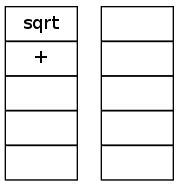
\includegraphics[scale=0.5]{images/stack-3.png}
  }
  \only<5>{
    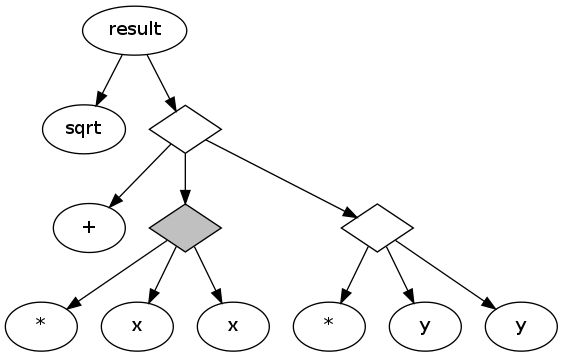
\includegraphics[scale=0.25]{images/vm-5.png}
    \hspace{.3in}
    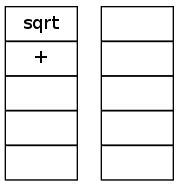
\includegraphics[scale=0.5]{images/stack-3.png}
  }
  \only<6>{
    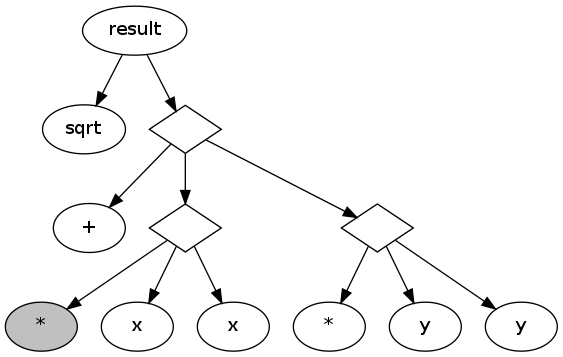
\includegraphics[scale=0.25]{images/vm-6.png}
    \hspace{.3in}
    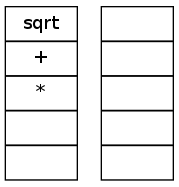
\includegraphics[scale=0.5]{images/stack-4.png}
  }
  \only<7>{
    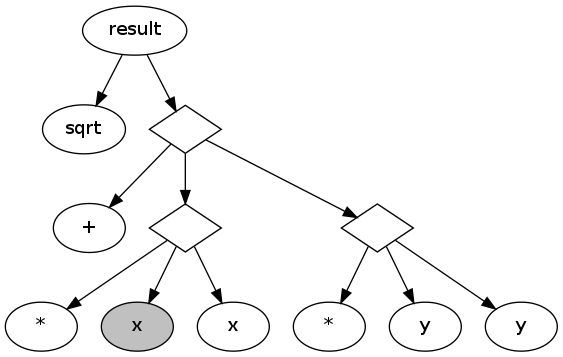
\includegraphics[scale=0.25]{images/vm-7.png}
    \hspace{.3in}
    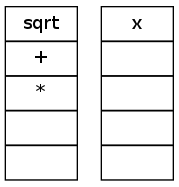
\includegraphics[scale=0.5]{images/stack-5.png}

    \texttt{push(x)}
  }
  \only<8>{
    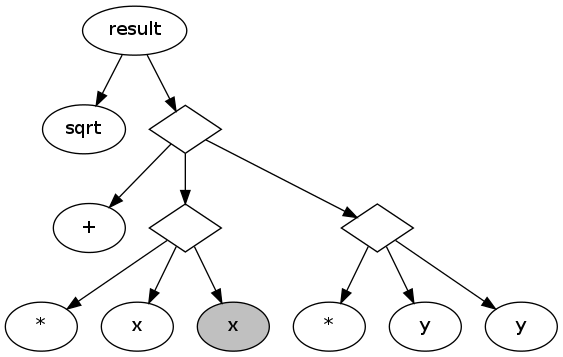
\includegraphics[scale=0.25]{images/vm-8.png}
    \hspace{.3in}
    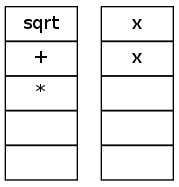
\includegraphics[scale=0.5]{images/stack-6.png}

    \texttt{push(x); push(x)}
  }
  \only<9>{
    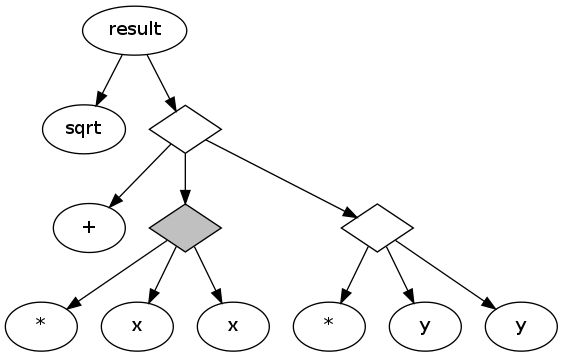
\includegraphics[scale=0.25]{images/vm-5.png}
    \hspace{.3in}
    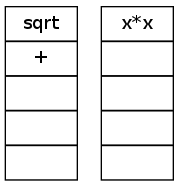
\includegraphics[scale=0.5]{images/stack-7.png}

    \texttt{push(x); push(x); multiply}
  }
  \only<10>{
    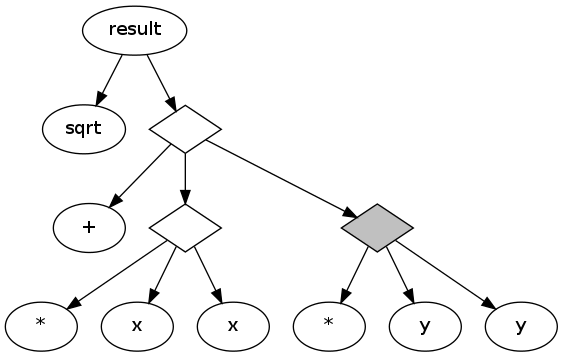
\includegraphics[scale=0.25]{images/vm-9.png}
    \hspace{.3in}
    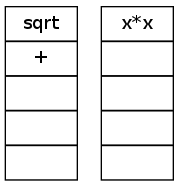
\includegraphics[scale=0.5]{images/stack-7.png}

    \texttt{push(x); push(x); multiply}
  }
  \only<11>{
    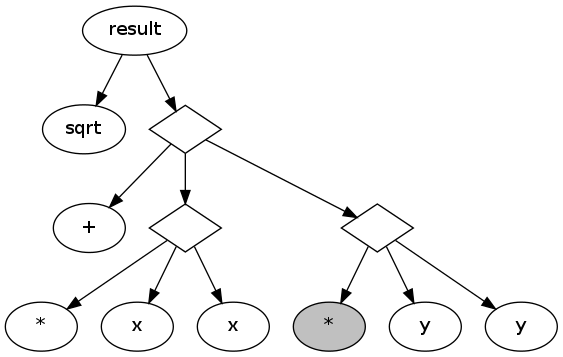
\includegraphics[scale=0.25]{images/vm-10.png}
    \hspace{.3in}
    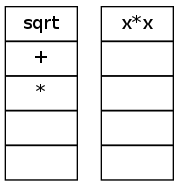
\includegraphics[scale=0.5]{images/stack-8.png}

    \texttt{push(x); push(x); multiply}
  }
  \only<12>{
    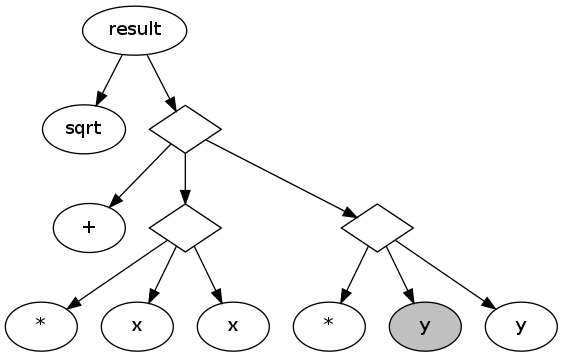
\includegraphics[scale=0.25]{images/vm-11.png}
    \hspace{.3in}
    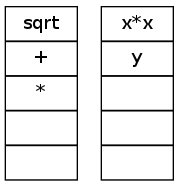
\includegraphics[scale=0.5]{images/stack-9.png}

    \texttt{push(x); push(x); multiply;\\push(y);}
  }
  \only<13>{
    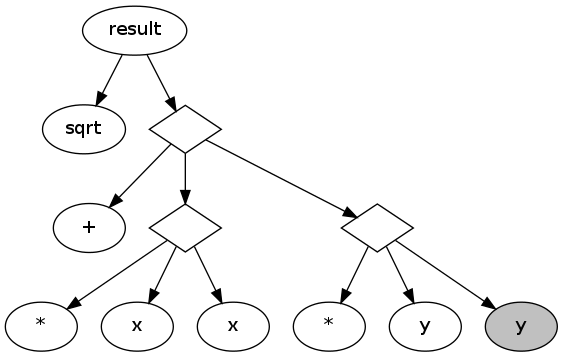
\includegraphics[scale=0.25]{images/vm-12.png}
    \hspace{.3in}
    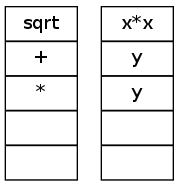
\includegraphics[scale=0.5]{images/stack-10.png}

    \texttt{push(x); push(x); multiply;\\push(y); push(y);}
  }
  \only<14>{
    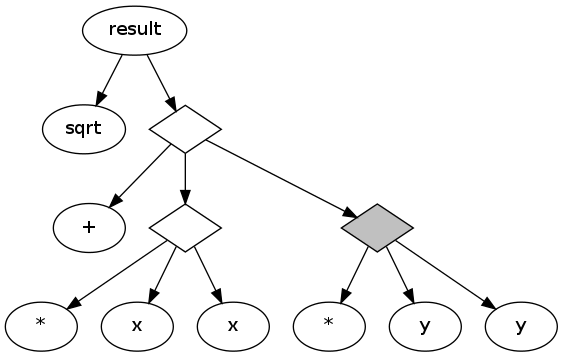
\includegraphics[scale=0.25]{images/vm-9.png}
    \hspace{.3in}
    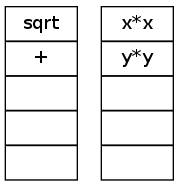
\includegraphics[scale=0.5]{images/stack-11.png}

    \texttt{push(x); push(x); multiply;\\push(y); push(y); multiply;}
  }
  \only<15>{
    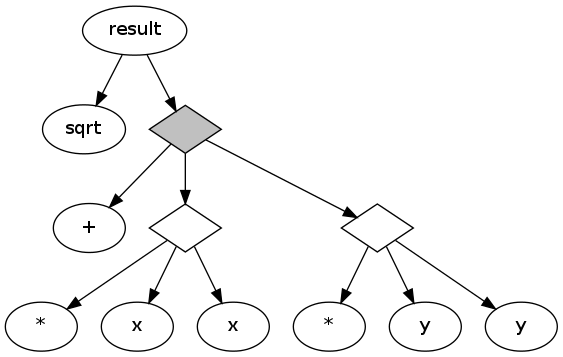
\includegraphics[scale=0.25]{images/vm-3.png}
    \hspace{.3in}
    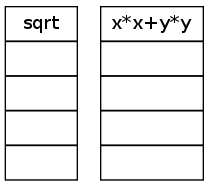
\includegraphics[scale=0.5]{images/stack-12.png}

    \texttt{push(x); push(x); multiply;\\push(y); push(y); multiply;\\plus;}
  }
  \only<16>{ 
    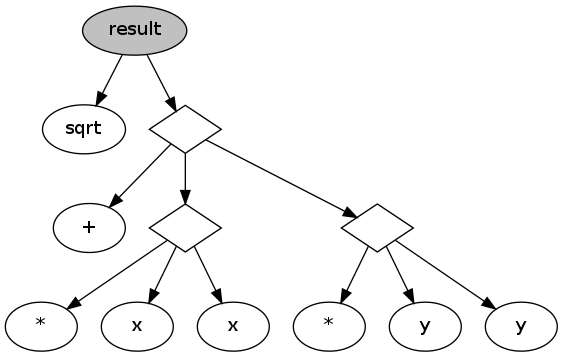
\includegraphics[scale=0.25]{images/vm-1.png}
    \hspace{.3in}
    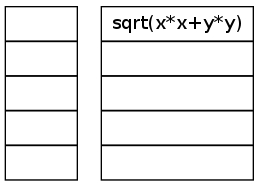
\includegraphics[scale=0.5]{images/stack-13.png}

    \texttt{push(x); push(x); multiply;\\push(y); push(y); multiply;\\plus; sqrt;}
  }
\end{frame}

\begin{frame}
  \frametitle{Core虚拟机的实现}
  \framesubtitle{标量原语SP的翻译}
  内建标量函数被直接翻译成C表达式或函数调用

  \texttt{+ a b $\rightarrow$  (a + b)}\\
  \texttt{exp n $\rightarrow$ exp(n)}
\end{frame}

\begin{frame}
  \frametitle{Core虚拟机的实现}
  \framesubtitle{向量原语VP的翻译}
  向量原语VP的翻译过程采用原语框架实例化实现。
  \begin{itemize}
    \item 原语框架
    \item 框架实例化
  \end{itemize}
\end{frame}

\begin{frame}
  \frametitle{向量原语VP的翻译}
  \framesubtitle{原语框架}
  map原语框架
  \lstinputlisting[language=C]{listings/map-skeleton.c}
\end{frame}

\begin{frame}
  \frametitle{向量原语VP的翻译}
  \framesubtitle{框架实例化}
  map原语实例化
  \lstinputlisting[language=C]{listings/map-instance.c}
\end{frame}

\subsection{前端优化技术}
\frame{\tableofcontents[currentsection, currentsubsection]}
\begin{frame}
  \frametitle{优化技术}
  Rat程序的优化技术简历在Core语言之上。主要的优化技术包括:
  \begin{itemize}
    \item 存储空间优化
    \item 向量原语聚合(VP fusion)
    \item 向量原语重排(VP reorder)
  \end{itemize}
\end{frame}

\begin{frame}
  \frametitle{存储空间优化}
  逻辑上,每一个VP作用在一个向量上都会得到一个新的向量。
  向量要占用大量的存储器资源,对向量存储空间的优化利用意义重大。存储空间
  可以优化措施的情况包括:
  \pause
  \begin{itemize}
    \item 如果原有的向量不再被使用,那么它使用的内存区域就可以回收重用
    \item 某些VP的并行实现可以原地完成,或者某些条件下可以完成
    %% \item 向量literal在某些情况下不需要初始化内存空间
  \end{itemize}
\end{frame}

\begin{frame}
  \frametitle{存储空间优化}
  \framesubtitle{向量内存重用}
  对于Rat程序中的任意向量,在编译期都可以确定它生命周期终点。在这一点之后的时刻,
  该向量的数据不在会被使用,那么它所占用的空间可以分配给其他向量使用。
  \pause
  \lstinputlisting[language=Haskell]{listings/frag-16.hs}
  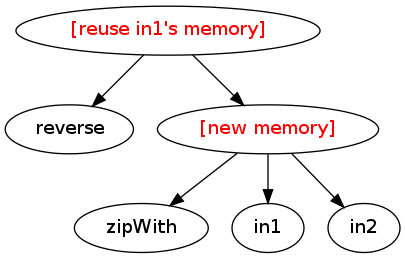
\includegraphics[scale=0.3]{images/reversezip.png}
\end{frame}

\begin{frame}
  \frametitle{存储空间优化}
  \framesubtitle{原地并行VP}
  向量原语的原地并行可执行能力如下表
  \begin{table}
    \caption{各向量原语的原地并行执行能力}
    \begin{tabular}{|l|l||l|l|}
      \hline
      map & yes & scale & 仅当内存缩小时\\
      \hline
      slice & yes & scan & no\\
      \hline
      compact & 需要同步 & sort & no\\
      \hline
      sparse & no & zip & yes\\
      \hline
      permute & 需要同步 & random & yes\\
      \hline
    \end{tabular}
  \end{table}
\end{frame}

%% \begin{frame}
%%   \frametitle{存储空间优化}
%%   \framesubtitle{向量literal免初始化}
%%   某些VP的调用中,出现在特定位置的向量literal可以不用初始化内存空间。\\
%%   \texttt{b = map f [1 .. 10000]}\\
%%   FIXME:这一张可以删掉
%% \end{frame}

\begin{frame}[t]
  \frametitle{向量原语聚合~VP fusion}
  向量原语聚合旨在合并相邻的VP,以提高执行效率。
  \lstinputlisting[language=Haskell]{listings/frag-12.hs}
  \begin{figure}
    \caption{VP fusion实例}
    \includegraphics<1>[scale=0.4]{images/vp-fusion-1.png}
    \includegraphics<2>[scale=0.4]{images/vp-fusion-2.png}
  \end{figure}
\end{frame}

\begin{frame}[t]
  \frametitle{向量原语重排~VP reorder}
  向量原语重排旨在交换可以换序的VP,以提高执行效率
  \lstinputlisting[language=Haskell]{listings/frag-12.hs}
  \begin{figure}
    \caption{VP reorder实例}
    \includegraphics<1>[scale=0.4]{images/vp-reorder-1.png}
    \includegraphics<2>[scale=0.4]{images/vp-reorder-2.png}
  \end{figure}
\end{frame}

\subsection{后端实现技术}
\frame{\tableofcontents[currentsection, currentsubsection]}

\begin{frame}
  \frametitle{Rat后端实现方案}
  \begin{figure}
    \caption{Rat后端结框图}
    \includegraphics<1>[scale=0.3]{images/backend.png}
    \includegraphics<2>[scale=0.3]{images/backend-gpu.png}
  \end{figure}
\end{frame}

\begin{frame}
  \frametitle{Runtime System}
  \framesubtitle{Task Scheduler}
  Task Scheduler的功能:
  \begin{itemize}
    \item 任务的划分
    \item 子任务的调度与分派
    \item 结果的收集与合并
    \item 管理运行于不同设备任务之间的并行执行或流水化执行
  \end{itemize}
\end{frame}

\begin{frame}
  \frametitle{Runtime System}
  \framesubtitle{Resource Manager}
  Resource Manager的功能:
  \begin{itemize}
    \item 管理可用设备(CPU,GPU ...)
    \item 管理向量内存的分配与回收
    \item 对于标量内存执行采用垃圾回收机制
  \end{itemize}
\end{frame}

\begin{frame}
  \frametitle{Runtime System}
  \framesubtitle{VP Driver}
  VP Driver是在不同硬件上定义的抽象功能接口,提供向量原语的具体实现。
  \begin{figure}
    \caption{Nvidia GPU线程模型}
    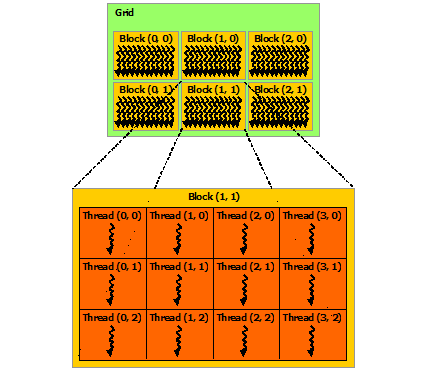
\includegraphics[scale=0.4]{images/grid-of-thread-blocks.png}
  \end{figure}
\end{frame}

\begin{frame}
  \frametitle{VP Driver的GPU实现}
  对于Rat提供的向量原语,有的已经在CUDPP\footnote{http://code.google.com/p/cudpp/}中有高效实现。
  剩余的原语的实现过程也比较直观。
  \begin{table}
    \caption{VP的GPU实现}
    \begin{tabular}{|l|l||l|l|}
      \hline
      map & ratMap & scale & ratCopy\\
      \hline
      slice & ratCopy & scan & cudappScan\\
      \hline
      compact & cudppCompact & sort & cudppSort\\
      \hline
      sparse & ratCopy & zip & \\
      \hline
      permute & ratCopy & random & cudppRand\\
      \hline
    \end{tabular}
  \end{table}
\end{frame}

\subsection{后端优化技术}
\frame{\tableofcontents[currentsection, currentsubsection]}
\begin{frame}
  \frametitle{后端优化技术}
  Rat的后端实现平台为Nvidia GPU,主要优化措施包括:
  \begin{itemize}
    \item 子程序并行执行
    \item GPU访存操作优化
  \end{itemize}
\end{frame}

\begin{frame}
  \frametitle{子程序并行执行}
  \begin{columns}
    \begin{column}{0.5\textwidth}
      为了提高整个程序的并行度,在硬件允许的情况下,尽量使CPU与GPU同时工作。
      \begin{itemize}
        \item GPU端的kernel调用采用异步模式
        \item 重叠Host-Device之间的数据传输与kernel执行
      \end{itemize}
    \end{column}
    \begin{column}{0.5\textwidth}
      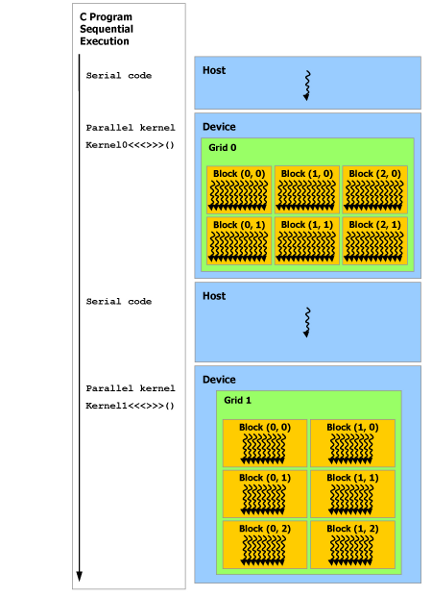
\includegraphics[scale=0.35]{images/heterogeneous-programming.png}
    \end{column}
  \end{columns}
  \pause
  \alert{“无副作用”}:可以任意选取子程序并行执行,不影响程序正确性。
\end{frame}

\begin{frame}
  \frametitle{GPU访存操作优化}
  要采用的访存优化措施主要包括:
  \begin{itemize}
    \item Coalesced Access to Global Memory
    \item Utilizing Shared Memory
  \end{itemize}
\end{frame}

\begin{frame}
  \frametitle{GPU访存操作优化}
  \framesubtitle{Coalesced Access to Global Memory}
  GPU上对于global memory的Coalesced Access可以在一次L1 cache transection内完成。
  \begin{itemize}
    \item 分配向量内存时对齐地址
    \item 分配kernel线程时匹配线程数目与数据块大小
  \end{itemize}
  \begin{figure}
    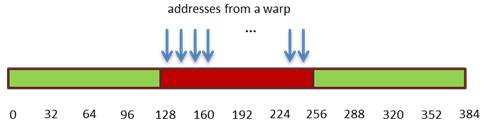
\includegraphics[scale=0.4]{images/coalesced-access.png}\\
    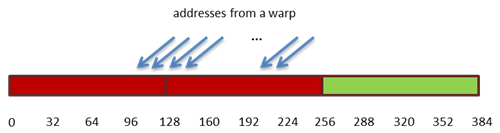
\includegraphics[scale=0.4]{images/unaligned-sequential-addresses.png}
  \end{figure}
\end{frame}

\begin{frame}
  \frametitle{GPU访存操作优化}
  \framesubtitle{Utilizing Shared Memory}
  位于同一个block的线程共享一块片上存储器shared memory,它的访问速度远远超过global memory
  \begin{itemize}
    \item 对于对源操作数读取次数大于1的操作,先将数据传送到shared memory再执行计算
    \item 对于fold操作,先在shared memory中进行局部reduce的性能远远超过全局reduce
  \end{itemize}
\end{frame}

%% chap 4
\section{课题状况}
\frame{\tableofcontents[currentsection]}
\begin{frame}
  \frametitle{Rat实现情况}
  Rat语言的实现正处于工作当中……
  \begin{table}
    \caption{Rat 语言各个组件实现情况}
    \begin{tabular}{|l|l|l|}
      \hline
      \multirow{3}{*}{前端} & Lexer & finished\\
      \cline{2-3}
      & Parser & finished\\
      \cline{2-3}
      & Type Checker & in progress\\
      \hline
      \multirow{3}{*}{后端} & Task Scheduler & in progress\\
      \cline{2-3}
      & Resource Manager & finished\\
      \cline{2-3}
      & \alert{VP Driver} & finished\\
      \hline
    \end{tabular}
  \end{table}
\end{frame}

\begin{frame}
  \Huge{the end}
\end{frame}

\end{document}
